% !TEX encoding = UTF-8 Unicode
% !TEX root = ..\main.tex
% !TEX spellcheck = en-US



% DEFINITION AND CHALLENGES, HOW IT RELATES TO THIS THESIS

% LINKING WORDS ARE IMPORTANT; similarly, in addition, also, again
% Disagreements; however, on the otehr hand, conversely, nevertheless

% Structure:

% - Introduction/definition of topic
% - 

\chapter{State-of-the-Art}
This chapter presents state-of-the-art topics which are relevant to this project. Section \ref{sec:2-TD} presents the technical debt with definitions, causes, and management tools. Section \ref{sec:2-SQ} looks into the topic of software quality and the relevant attributes. Section \ref{sec:2-SLC} presents the software life cycle along with the different development methodologies. Section \ref{sec:2-SA} presents software architecture. Section \ref{sec:2-SE} presents software evolution and maintenance.
Section \ref{sec:2-SR} takes a look into software reuse. Section \ref{sec:2-Refactoring} presents refactoring. Section \ref{sec:2-CM} presents configuration management. Lastly, Section \ref{sec:2-ES} will take a closer look at embedded systems and software.


\section{Technical Debt}
\label{sec:2-TD}
The concept of technical debt was first introduced by Ward Cunningham in 1992 to communicate technical problems with non-technical stakeholders\cite{p29-cunningham}. The concept was used to describe the system design trade-offs that are made everyday. To deliver business functionality as quickly as possible, \textit{'quick and dirty'} decisions had to be made, which affected the future development activities. Furthermore, Cunningham describes technical debt as \textit{"shipping first time code is like going into debt. A little debt speeds development as long as it is paid back promptly with a rewrite"}. As the time goes, technical debt accumulates \textit{interest}, leading to increased costs of a software system\cite{p31-guo,p35-klinger}. Li et al.\cite{li2015systematic} defines interest as \textit{the extra effort needed to modify the part of the software system that contains technical debt}. However, not all debts are necessarily bad. A small portion of debt may help developers speed up the development process, resulting in short-term benefits\cite{p31-guo}. 

%% The costs of technical debt
\begin{figure}[ht!]
	\centering
	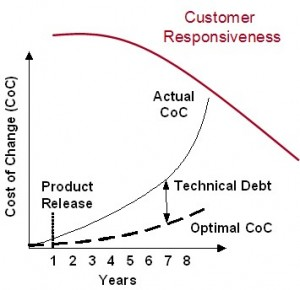
\includegraphics[width=0.8\textwidth]{images/techdebtCurve.jpg}
	\caption{The Technical Debt Curve\cite{jim-highsmith}}
	\label{fig:techDebtCurve}
\end{figure}

Figure \ref{fig:techDebtCurve} illustrates the effects of technical debt growth in a system.

%%%

\subsection{Definitions of Technical Debt}
McConnell\cite{url-mcconnell} describes technical debt as \textit{a design or construction approach that is expedient in the short term but that creates a technical context in which the same work will cost more to do later than it would cost to do now (including the increased cost over time)}. He splits the term into two categories based on how they are incurred; technical debt that is incurred \textit{intentionally}, and technical debt that is incurred \textit{unintentionally}. For instance, unintentional debt accumulates when a junior software developer writes low quality code due to lack of knowledge and experience. Intentional debt commonly occurs when an organization makes a decision to optimize for the present rather than the future. These type of decisions results in shortcuts being taken to solve a problem.

Fowler\cite{url-fowler} presents a more formal explanation of how technical debt can occur. He categories technical debt into a quadrant with two dimensions, which he calls the \textit{"Technical Debt Quadrant"}. As seen in the Figure \ref{fig:techDebtQuad}, the debt is grouped into four categories: 

\begin{figure}[ht!]
	\centering
	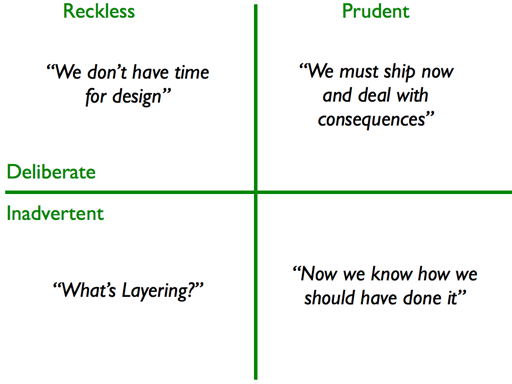
\includegraphics[width=0.8\textwidth]{images/techDebtQuadrant.png}
	\caption{Fowler's Technical Debt Quadrant}
	\label{fig:techDebtQuad}
\end{figure}

\begin{itemize}
	\item \textbf{Reckless/Deliberate debt}: The team feels time pressure, and takes shortcuts intentionally without any thoughts on how to address the consequences in the future.
	\item \textbf{Reckless/Inadvertent debt}: Best practices for code and design is ignored, and a big mess in the code base is made.
	\item \textbf{Prudent/Deliberate debt}: : The value of taking shortcuts is worth the cost of incurring debt in order to meet a deadline. The team is aware of the consequences, and has a plan in place to address them in the future. 
	\item \textbf{Prudent/Inadvertent debt}: Software development process is as much learning as it is coding. The team can deliver a valuable software with clean code, but in the end they may realize that the design could have been better.
\end{itemize}

Krutchen et al.\cite{krutchen} divides technical debt into two categories; \textit{Visible debt}, that is visible for everyone. It contains elements such as new functionality to add, and defects to fix. \textit{Invisible debt} is the other category, debt that is only visible to software developers. Figure \ref{fig:techDebtLandscape} illustrates a map of the \textit{"Technical Debt Landscape"}, in which distinguish visible and invisible elements. On the left side of Figure \ref{fig:techDebtLandscape}, technical debt mostly affects evolvability of the software system, while on the right side, technical debt mainly affects maintainability.

\begin{figure}[ht!]
	\centering
	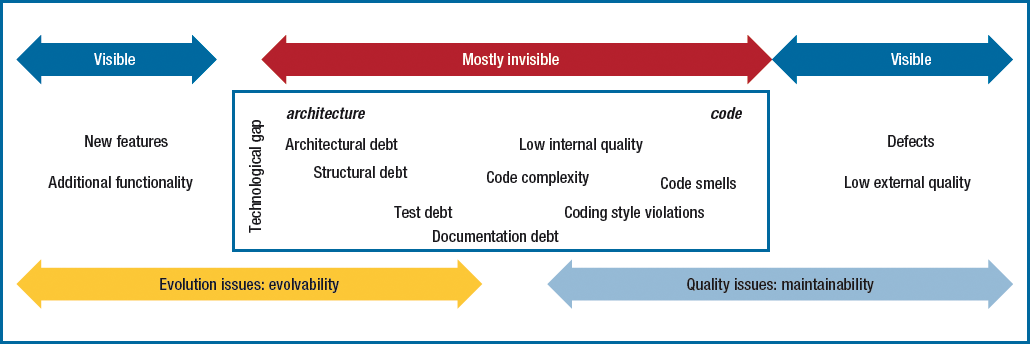
\includegraphics[width=1.0\textwidth]{images/techDebtLandscape.png}
	\caption{Technical Debt Landscape}
	\label{fig:techDebtLandscape}
\end{figure}

\subsection{Comparison with Financial Debt}
Technical debt has many similar characteristics to financial debt\cite{p50-allman,Zazworka:2011:PDD:1985362.1985372}:
\begin{itemize}
	\item You take a loan that has to be repaid later
	\item You usually repay the loan with interest
	\item If you can not pay back, a very high cost will follow. For example, you can loose your house or car.
\end{itemize}

Like financial debt, technical debt accrues interest over time which comes in the form of extra effort that has to be dedicated in future development\cite{p31-guo,p35-klinger}. Stakeholders can choose to continue paying interest, or to reduce future interest payments by refactoring the problem\cite{url-fowler}. 


However, if the debt is not repaid, the development may slow down, resulting in software project failure or bankruptcy\cite{p50-allman}. Moreover, there are some differences between financial debt and technical debt. The debt has to be repaid eventually, but not on any fixed schedule\cite{p50-allman}. This means that some debts may never have to be paid back, depending on the interest and the cost of paying back the debt\cite{foser076-brown}.


\subsection{Causes and Effects of Technical Debt}
Multiple studies have tried to analyze the reason for companies to incur technical debt.

Klinger et al.\cite{p35-klinger} conducted an industrial case study at IBM where four technical architects with different backgrounds were interviewed. The goal was to examine how decisions to incur debt were taken, and the extent to which the debt provided leverage\cite{p35-klinger}. The study revealed that the company failed to assess the impact of intentionally incurring debt on projects. Decisions regarding technical debt were rarely quantified. The study also revealed big organizational gaps among the business, operational, and technical stakeholders. When the project team felt pressure from the different stakeholders, technical debt decisions were made without quantifications of possible impacts.

Lim et al.\cite{lim-taksande} pointed out that technical debt is not always the result of poor developer disciplines, or sloppy programming. It can also include intentional decisions to trade off competing concerns during business pressure. Furthermore, Li et al. explains that technical debt can be used in short term to capture market share and to collect customers feedback early. In the long term, technical debt tended to be negative. These trade-offs included increased complexity, reduced performance, low maintainability, and fragile code. This led to bad customer satisfaction and extra working hours. In many cases, the short term benefits of technical debt outweighed the future costs.

Guo et al.\cite{guo2011tracking} studied the effects of technical debt by tracking a single delayed maintenance task in a real software project throughout its life-cycle, and simulated how managing technical debt can impact the project result. The results indicated that delaying the maintenance task would have almost tripled the costs, if it had been done later.

Siebra et al.\cite{p247-siebra} carried out an industrial case study where they analyzed documents, emails, and code files. Additionally, they interviewed multiple developers and project managers. The case study revealed that technical debt were mainly taken by strategic decisions. Furthermore, they commented out that using a unique specialist could lead the development team to solutions that the specialist wanted and believe were correct, leading the team to incur debt. The study also identified that technical debt can both increase and decrease the amount of working hours.

Zazworka et al.\cite{zazworka2011investigating} studied the effects of god classes and technical debt on software quality. God classes are examples on bad coding, and therefore includes a possibility for refactoring\cite{Zazworka:2011:PDD:1985362.1985372}. The results indicated that god classes require more maintenance effort including bug fixing and changes to software that are considered as a cost to software project. In other words, if developers desire higher software quality, then technical debt needs to be addressed closely in the development process.

Buschmann\cite{buschmann2011pay} explained three different stories of technical debt effects. In the first case, technical debt accumulated in a platform started had growth to a point where development, testing, and maintenance costs started to increase dramatically. Additionally, the components were hardly usable. In the second case, developers started to use shortcuts to increase the development speed. This resulted in significant performance issues because an improper software modularization reflected organizational structures instead of the system domains. It ended up turning in to economic consequences. In the last case, an existing software product experienced increased maintenance cost due to architectural erosion. However, management analyzed that re-engineering the whole software would cost more than doing nothing. Management decided not to do anything to technical debt, because it was cheaper from a business point-of-view.

Codabux et al.\cite{p8-codabux} carried out an industrial case study where the topic was agile development focusing on technical debt. They observed and interviewed developers to understand how technical debt is characterized, addressed, prioritized, and how decisions led to technical debt. Two subcategories of technical debt were commonly described in this case study; infrastructure and automation debt. 

The studies indicates that the causes and effects of technical debt are not always caused by technical reasons. technical debt can be the result of intentional decisions made by the different stakeholders. Incurring technical debt may have short-term positive effects such as time-to-market benefits. Not paying down technical debt can result economic consequences, or quality issues in the long-run. The allowance of technical debt can facilitate product development for a period, but decreases the product maintainability in the long-term. However, there are some times where short-term benefits overweight long-term costs\cite{guo2011tracking}. 

Furthermore, the studies points out that several types of technical debt are related to software life-cycle phases. The effects of taking shortcuts can happen in several stages of software life-cycle. Table \ref{tab:subcategories} lists the types of technical debt that has been identified in the literature.

\begin{table}
	\centering
	\begin{tabular}{ | p{5cm} | p{8cm} |}
	\hline
	\textbf{Subcategory} & \textbf{Definition} \\ \hline
	Architectural debt\cite{li2015systematic,p8-codabux,foser076-brown} & Architectural decisions that make compromises in some of the quality attributes, such as modifiability. \\ \hline
	Code debt\cite{li2015systematic,foser076-brown,tom2013exploration} & Poorly written code that violates best coding practices and guidelines, such as code duplication. \\ \hline
	Defect debt\cite{li2015systematic,tom2013exploration} & Defect, failures, or bugs in the software. \\ \hline
	Design debt\cite{li2015systematic,Zazworka:2011:PDD:1985362.1985372,foser076-brown} & Technical shortcuts that are taken in design.\\ \hline
	Documentation debt\cite{li2015systematic,foser076-brown,Zazworka:2013:CSE:2460999.2461005} & Refers to insufficient, incomplete, or outdated documentation in any aspect of software development.\\ \hline
	Infrastructure debt\cite{li2015systematic,tom2013exploration,p8-codabux} & Refers to sub-optimal configuration of development-related processes, technologies, and supporting tools. An example is lack of continuous integration.\\ \hline
	Requirements debt\cite{li2015systematic,Zazworka:2013:CSE:2460999.2461005} & Refers to the requirements that are not fully implemented, or the distance between actual requirements and implemented requirements.\\ \hline
	Test debt\cite{li2015systematic,Zazworka:2013:CSE:2460999.2461005,foser076-brown} & Refers to shortcuts taken in testing. An example is lack of unit tests, and integration tests.\\
	\hline
	\end{tabular}
	\caption{Types of Technical Debt} \label{tab:subcategories}
\end{table}

\subsection{Current Strategies and Practices for Managing Technical Debt}
Managing technical debt compromises the actions of identifying the debt and making decisions about which debt should be repaid\cite{foser076-brown,krutchen,url-mcconnell}. This section examines some methods that has been proposed by several authors.

Brown et al.\cite{foser076-brown} proposed open research questions to understand the need to manage technical debt. The questions includes refactoring opportunities, architectural issues, identifying dominant sources of technical debt, and identifying issues that arise when measuring technical debt.

%Lim.et al - 4 strategies
Lim et al.\cite{lim-taksande} suggested four strategies for managing technical debt. The first strategy is to do nothing because the technical debt may never be visible to the customer. The second strategy is to use a risk management approach to evaluate and prioritize technical debts cost and value by allocating 5-10\% of each release cycle to address technical debt. The third strategy is to include the customers and non-technical stakeholders to technical debt decisions. Finally, the last strategy suggests to track technical debt items using tools like a Wiki, or a backlog.

%Codabux
Codabux et al.\cite{p8-codabux} suggested best practices such as refactoring, repackaging, re-engineering, and developing unit tests to manage technical debt. Moreover, they also propose that having dedicated teams with the purpose of reducing technical debt, while the product development team devote 20\% of their effort toward technical debt reduction.
	
%Portifolio management (guo, zazworka (priorizing design debt investment opportunities))
Guo et al.\cite{p31-guo} suggested using of portfolio management for technical debt management. This approach collects technical debt items to a \textit{"Technical Debt List"} (Technical DebtL). TDL is used to pay technical debt back based on its cost and value. Three activities support the TDL. The first activity is Technical Debt Identification. Technical Debt Identification uses several tools to identify technical debt items, in which are automatically placed in the TDL. The second activity is Technical Debt Estimation. Each item in the list is assigned the estimates for the debt principal, and the interest. The third activity, Decision Making, is used to determine which debts should be addressed first, and when they should be addressed.

%Quantifying technical debt - Nugraho
Nugraho et al.\cite{p1-nugraho} proposed an approach to quantify technical debt and its interest by using a software quality assessment method. This method rates the technical quality of a system in terms of the quality characteristics of ISO/IEC 9126. 

%Krutchen (define tech debt in your backlog)
Krutchen et al.\cite{krutchen} suggested listing debt-related tasks in a common backlog during release and iteration planning. Figure \ref{fig:fourColorBacklog} illustrates how these elements can be organized in a backlog. Moreover, Krutchen mentioned that project backlogs often contain the green elements. The rest are seen rarely, especially the black elements, they are nowhere to be found.


\begin{figure}[ht!]
	\centering
	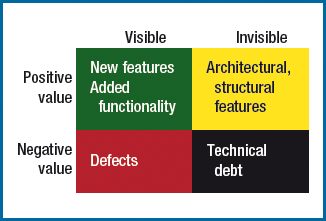
\includegraphics[width=0.8\textwidth]{images/fourColorBacklog.png}
	\caption{The Colors Reconcile Four Types of Possible Improvements.}
	\label{fig:fourColorBacklog}
\end{figure}

SonarQube is an open source application for quality management\cite{sonarsource2013sonarqube}. It manages the results of various code analysis tools, and is used to analyze and measure a projects technical quality. Technical debt is computed based on the SQALE (Software Quality Assessment based on Life-cycle Expectations) methodology\cite{letouzey2012sqale}. SQALE is a method for assessing technical debt in a project. It is based on tools that analyze the source code of the project, looking at different types of errors such as mismatched indentation, and different naming conventions. Each error is assigned a score based on how much work it would take to fix that error. The analysis gives a total sum of technical debt for the entire project.



%%%%%%%%%%%%%%%%%%%%

% Kvalitet

%%%%%%%%%%%%%%%%%%%%%

\section{Software Quality}
\label{sec:2-SQ}
Software Quality (SQ) is defined as \textit{an effective software process applied in a manner that creates a useful product that provides measurable value for those who produce it and those who use it}\cite{Pressman:2009:SEP:1593949}. ISO/IEC 9126-2001 is an international standard for evaluating software\cite{ISOIEC9126}. It is currently one of the most widespread quality standards\cite{trienekens2010quality}. The standard defines quality as \textit{the totality of characteristics of an entity that bear on its ability to satisfy stated and implied needs}. Additionally, ISO/IEC 9126-2001 offers a valuable conceptual framework for SQ, where it makes a distinction between \textit{"quality in use"}, \textit{"external quality"}, and \textit{"internal quality"}\cite{ISOIEC9126,trienekens2010quality}. \textit{Quality in use} is the users view of the quality of a system. \textit{External quality} reflects the dynamic aspect of a software application, and is subdivided into six quality characteristics. \textit{Internal quality} is reflected by a subdivision of the six external quality characteristics into internal quality attributes.

Table \ref{tab:qattribute} describes the quality attributes, and their sub-characteristics (criteria).

\begin{table}[ht!]
	\centering
	\begin{tabular}{ | l | p{4cm} | p{6cm} |}
	\hline
	\textbf{Quality Attribute} & \textbf{Criteria} & \textbf{Description} \\ \hline
	Functionality 		&	Suitability, Accuracy, Interoperability, Security, Functionality compliance 	&	Ability of the system to do work for which it was intended. \\ \hline
	Reliability 		&	Maturity, Fault tolerance, Recoverability, Reliability compliance	&	Ability of the system to keep operating over time under certain conditions. \\ \hline
	Usability 			&	Understandability, Learnability, Operability, Attractiveness, Usability compliance 	 &	The capability of the software product to be understood, learned, and used by users. \\ \hline
	Efficiency 			&	Time behavior, Resource utilization, Efficiency compliance	 &	The capability of the software product to provide appropriate performance, relative to the amount of resources used, under stated conditions. \\ \hline
	Maintainability 	&	Analyzeability, Changeability, Stability, Testability, Maintainability compliance	 &	The capability of the software product to be modified in the future.\\ \hline
	Portability 		&	Adaptability, Installability, Co-existence, Replaceability, Portability compliance 	 &	The capability of the software product to be transferred from one environment to another. \\ \hline
	\end{tabular}
	\caption{The Sub-Characteristics Adopted by ISO/IEC 9126-2001} \label{tab:qattribute}
\end{table}





%%%%%%%%%%%%%%%%%%%%%%%%%%%%%%%%%%%%%%%%%%%%%%%%%%%%%%%%%%%%%%%%%%%%%%%%%%%%%%%%%%%%%%

			% SOFTWARE ARCHITECTURE

%%%%%%%%%%%%%%%%%%%%%%%%%%%%%%%%%%%%%%%%%%%%%%%%%%%%%%%%%%%%%%%%%%%%%%%%%%%%%%%%%%%%%%
\section{Software Architecture}
\label{sec:2-SA}
Bass et al.\cite{Bass:2012:SAP:2392670} defines software architecture as following: 

\begin{displayquote}
\textit{The software architecture of a system is the set of structures needed to reason about the system, which compromise software elements, relations among them, and properties of both.}
\end{displayquote}

The architecture of a software is one of the most important artifacts within the systems life cycle\cite{Bass:2012:SAP:2392670,knodel2006static}. Architectural design decisions that are made during the design phase, affect the systems ability to accept changes and to adapt to changing market requirements in the future. As the design decisions are made early, it will directly affect the evolution and maintenance phase\cite{Pressman:2009:SEP:1593949}, activities that consumes a big part of the systems lifespan\cite{Vliet:2008:SEP:1481475}. The issues of software architecture has long been a concern for those building and evolving large software systems\cite{perry1997state}.

Software architecture can be seen from two standpoints\cite{mooc}; \textit{prescriptive and descriptive architecture}. The \textit{prescriptive architecture} of a system captures the design decisions made prior to the construction. This is normally called as-conceived software architecture. \textit{Descriptive architecture} describes how the system has actually been build, called for as-implemented software architecture. 

As the system evolves, it is ideal that the prescriptive architecture is modified first. In practice, the system - the descriptive architecture - is often directly modified\cite{Bass:2012:SAP:2392670}. This may be due to developers sloppiness, short deadlines, or lack of documented prescriptive architecture. These principles introduces two new concepts; \textit{architectural drift} and \textit{architectural erosion}\cite{Bass:2012:SAP:2392670}. Architectural drift occurs when the documents are updated according to the implementation. The software architecture ends up as an architecture without vision and direction. Architectural erosion occurs when the implementation drifts away from the planned architecture. 

System requirements can be categorized as \textit{functional requirements}, \textit{quality attribute requirements} (QA requirements), and \textit{constraints}\cite{Bass:2012:SAP:2392670}. \textit{Functional requirements} states what a system must do. \textit{QAs} are the non-functional requirements of a system. \textit{Constraints} is a design decision with zero degrees of freedom. Moreover, long-term responsiveness of a system can be achieved by providing a solution of a system that would enable and achieve systems driving QA. 

As a final step in the architecture design phase, more and more organizations are evaluating their design decisions using Architecture Trade-off Analysis Model\cite{Bass:2012:SAP:2392670,sherman2008quality}. The goal of the ATAM is to understand the consequences of architectural decisions with respect to the quality attribute requirements of the system.





%%%%%%%%%%%%%%%%%%%%%%%%%%%%%%%%%%%%%%%%%%%%%%%%%%%%%%%%%%%%%%%%%%%%%%%%%%%%%%%%%%%%%%

		% SOFTWARE MAINTENANCE AND EVOLUTION

%%%%%%%%%%%%%%%%%%%%%%%%%%%%%%%%%%%%%%%%%%%%%%%%%%%%%%%%%%%%%%%%%%%%%%%%%%%%%%%%%%%%%%
\section{Software Evolution}
\label{sec:2-SE}
Increasingly, more and more software developers are employed to maintain and evolve existing systems instead of developing new systems from scratch\cite{Sommerville:2011:SE}. Software evolution is a process that usually takes place when the initial development of a software project is done and was successful\cite{Bennett:2000:SME:336512.336534}. The goal of software evolution is to incorporate new user requirements in the application, and adapt it to the existing application. Software evolution is important because it takes up to 85-90\% of organizational software costs\cite{Sommerville:2011:SE}. Software evolution is also important because technology tend to change rapidly.

Rajlich et al.\cite{Bennett:2000:SME:336512.336534} proposed a view of the software lifespan, as shown in Figure \ref{fig:lifespan-1}. This view divides the software lifespan into five stages with initial development as the first stage. The key contribution is to separate the maintenance phase into an evolution stage, followed by a service stage, and at last the phase-out stage.
\begin{description}
	\item[Initial development] produces the first version of the software from scratch.
	\item[Evolution] is the phase where significant changes to the software may be made. This could be addition of new features, correct previous mistakes, or adjust the software to new business requirements or technologies. Each change introduces a new feature or some other new property into the software.
	\item[Servicing] is the stage where relatively small, essential changes are allowed. The company considers how the software can be replaced. Legacy software is a term to describe software in this stage.
	\item[Phase-out] is the phase where software may still be used, but no further changes are being implemented. Users must work around any problems that they discover, or replace the software with something else.
	\item[Close-down] is when the managers or customers completely withdraw the system from production.
\end{description} 

\begin{figure}[ht!]
	\centering
	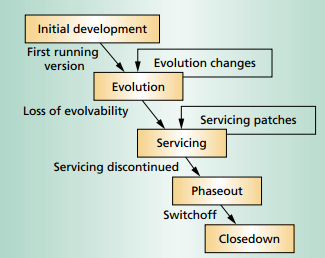
\includegraphics[width=0.8\textwidth]{images/lifespan-1.png}
	\caption{Software evolution process}
	\label{fig:lifespan-1}
\end{figure}

A variation of this process is the versioned stage model, as shown in Figure \ref{fig:lifespan-2}. When a software version is completed and released to the customer, the evolution continues with the company eventually releasing another version and only servicing the previous version. 

\begin{figure}[ht!]
	\centering
	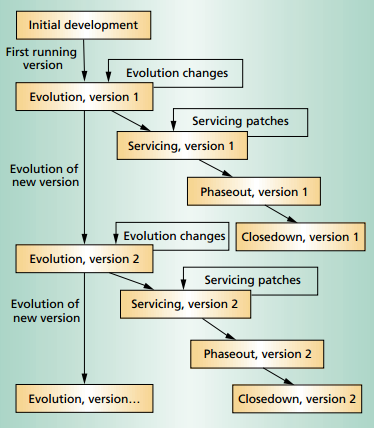
\includegraphics[width=0.8\textwidth]{images/lifespan-2.png}
	\caption{Software lifespan}
	\label{fig:lifespan-2}
\end{figure}

\subsection{Evolution Processes}
Software evolution usually starts with change proposals, which may be new requirements, existing requirements that have not been implemented, or bug reports from stakeholders. The process of implementing a change goes through these stages\cite{Sommerville:2011:SE} as shown in Figure \ref{fig:seProcess}.

The process starts with a set of proposed change requests. The cost and impact of the change is analyzed to decide whether to accept or deny the proposed changes. If the proposed changes are accepted, a new release of the system is planned. During release planning, all proposed changes such as fault repair, adaptation, and new functionality, are considered, to decide which changes to implement in the next version of the system. The changes are implemented and validated, and a new version of the system is released. The process ends with a new iteration with a set of proposed change requests for the next release. 

Sometimes, the need of urgent changes may appear, such as a serious system fault that must be repaired to allow normal operation. In these cases, the usual process will not be beneficial as it takes time. An emergency fix is usually made to solve the problem. A developer choose a quick and workable solution rather than the best solution. The trade-off is that the the requirements, the software design, and the code become inconsistent. As a system changes over time, it will have impact on the systems internal structure and complexity. Software evolution might cause poor SQ and erosion of software architecture over time\cite{Bass:2012:SAP:2392670}.

\begin{figure}[h!]
	\centering
	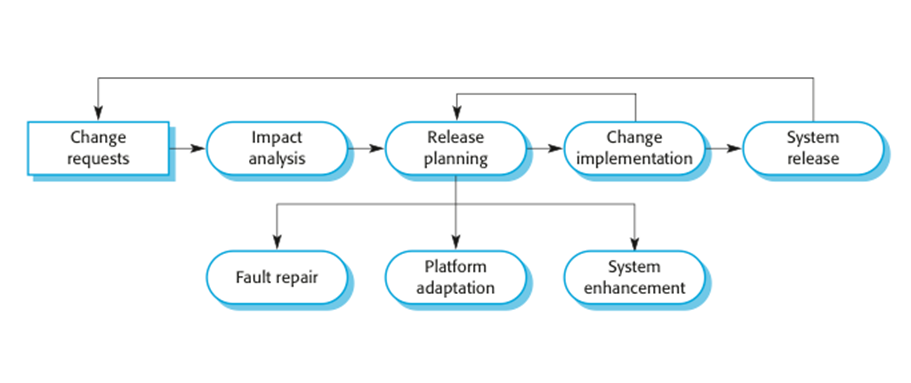
\includegraphics[width=0.8\textwidth]{images/SEprocess.png}
	\caption{Software evolution process}
	\label{fig:seProcess}
\end{figure}


\subsection{Software Maintenance}
IEEE 1219 defines software maintenance as follows\cite{720567}:
\begin{displayquote}
\textit{Modification of a software after delivery to correct faults, to improve performance or other attributes, or to adapt the product to a modified environment.}
\end{displayquote} 
Maintenance can be classified into four types\cite{Bennett:2000:SME:336512.336534,720567}.

\begin{itemize}
	\item Adaptive: Modification of a software product performed after delivery to keep a computer program usable in a changed or changing environment.
	\item Perfective: Modification of a software product after delivery to improve performance or maintainability.
	\item Corrective: Reactive modification of a software product performed after delivery to correct discovered faults.
	\item Preventive: Maintenance performed for the purpose of preventing problems before they occur.
\end{itemize}

According to van Vliet, the real maintenance activity is corrective maintenance\cite{Vliet:2008:SEP:1481475}. 50\% of the total software maintenance is spent on perfective, 25\% on adaptive maintenance, and 4\% on preventive maintenance. This leads to that 21\% of the total maintenance activity is corrective maintenance, the 'real' maintenance\cite{Vliet:2008:SEP:1481475}. This has not changed since the 1980s when Lientz and and Swanson conducted a study on software maintenance\cite{lientz1980software}. Their study found out that most severe maintenance problems were caused by poor documentation, demand from users for changes, poor meeting scheduled, and problems training new hires. Some other problem areas were lack of user understanding, user training, and that customers did not understand how the system worked.

\begin{figure}
	\centering
	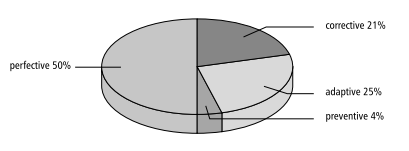
\includegraphics[width=0.8\textwidth]{images/maintenance.png}
	\caption{Distribution of maintenance activities\cite{Vliet:2008:SEP:1481475}}
	\label{fig:maintenanceActivities}
\end{figure}



%%%%%%%%%%%%%%%%%%%%%%%%%%%%%%%%%%%%%%%%%%%%%%%%%%%%%%%%%%%%%%%%%%%%%%%%%%%%%%%%%%%%%%

			% SOFTWARE REUSE

%%%%%%%%%%%%%%%%%%%%%%%%%%%%%%%%%%%%%%%%%%%%%%%%%%%%%%%%%%%%%%%%%%%%%%%%%%%%%%%%%%%%%%
\section{Software Reuse}
\label{sec:2-SR}
Software reuse is the process of using existing software artifacts, or knowledge, to create new software, rather than building it from scratch. Software reuse is a key method for improving software quality\cite{frakes1996software}. Software reuse can be specified in two directions, development \textit{for} reuse, and development \textit{with} reuse\cite{Slyngstad:2006:ESD:1159733.1159770}. Development \textit{for} reuse is related to components for reuse or system generalization. Development \textit{with} reuse is related to how existing components can be reused in new system.

Table \ref{tab:reusableComponents} lists several assets from a software project that can be reused\cite{frakes1996software}.
\begin{table}[H]
	\centering
	\begin{tabular}{ | l | l |}
	\hline
	1. architectures & 6. estimates \\ \hline
	2. source code & 7. human interfaces \\ \hline
	3. data & 8. plans \\ \hline
	4. designs & 9. requirements \\ \hline
	5. documentation & 10. test cases \\
	\hline
	\end{tabular}
	\caption{Reusable assets in software projects} \label{tab:reusableComponents}
\end{table}

Slyngstad et al.\cite{Slyngstad:2006:ESD:1159733.1159770} conducted an empirical study in Statoil ASA where they investigated developers views on software reuse. The results indicated that reuse include lower costs, shorter development time, higher quality of the reusable components, and a standardized architecture. These findings are very similar to the key benefits of reuse that Lim has described\cite{lim1994effects}. The quality of software artifacts increases every time the item is reused, because errors are discovered more frequently, making it easier to keep the artifact more stable\cite{sametinger1997software}.

Additionally, there can be problems associated with software reuse. A case study on a selected feature from self-driving miniature car development revealed that reuse of legacy, third party, or open source code, was one of the root causes for the accumulation of technical debt\cite{6974884}. Morisio et al.\cite{995420} identified three main causes of software reuse failure; not introducing reuse-specific processes, not modifying non-reuse processes, and not considering human factors, combined with lack of commitment by top management.

%%%%%%%%%%%%%%%%%%%%%%%%%%%%%%%%%%%%%%%%%%%%%%%%%%%%%%%%%%%%%%%%%%%%%%%%%%%%%%%%%%%%%%

			% REFACTORING

%%%%%%%%%%%%%%%%%%%%%%%%%%%%%%%%%%%%%%%%%%%%%%%%%%%%%%%%%%%%%%%%%%%%%%%%%%%%%%%%%%%%%%
\section{Refactoring}
\label{sec:2-Refactoring}
technical debt accumulates as developers write code\cite{Zazworka:2011:PDD:1985362.1985372}, and can be reduced by refactoring. Fowler defines refactoring as means of adjusting the design and architecture towards new requirements without changing the external behavior of a program in order to improve the quality of the system\cite{1999:RID:311424}. It is an act of improving the design and quality of an existing system\cite{Vliet:2008:SEP:1481475}. Most of the time spent on reducing technical debt is on refactoring activities itself. These activities includes planning the design and architecture, rewriting the code, and adjusting documentation\cite{Pressman:2009:SEP:1593949}. It is believed that refactoring improves software quality and developer productivity, by making it easier to understand and maintain software codes\cite{Kim:2012:FSR:2393596.2393655}, thus a way to manage the technical debt of a system. 

Table \ref{tab:refactorArtifacts} lists the software artifacts that refactoring applies to\cite{1265817}.

\begin{table}[ht!]
	\renewcommand{\arraystretch}{1.2}
	\centering	
	\begin{tabular}{p{0.6\textwidth}} \hline
		\textbf{Programs} \\Refactoring at the source code or program level. For example, extracting methods, and encapsulating fields. \\ \hline
		\textbf{Designs} \\
		Refactoring at design level, for example in the form of UML models. Design patterns, software architecture, and database schemas, are some examples on artifacts that can be refactored at this level. \\ \hline
		\textbf{Software Requirements} \\
		Refactoring at the level of requirements specification. For example, decomposing requirements into a structure of viewpoints. \\ \hline
	\end{tabular}
	\caption{Types of Software Artifacts that can be refactored.}
	\label{tab:refactorArtifacts}
\end{table}





%%%%%%%%%%%%%%%%%%%%%%%%%%%%%%%%%%%%%%%%%%%%%%%%%%%%%%%%%%%%%%%%%%%%%%%%%%%%%%%%%%%%%%
			
				% EMBEDDED SYSTEMS %

%%%%%%%%%%%%%%%%%%%%%%%%%%%%%%%%%%%%%%%%%%%%%%%%%%%%%%%%%%%%%%%%%%%%%%%%%%%%%%%%%%%%%%
\section{Embedded Systems}
\label{sec:2-ES}
Embedded systems are special-purpose computer systems designed to perform certain dedicated functions under certain constraints. For instance, an embedded system in an automobile provides specific functions as a subsystem for the car itself\cite{Crnkovic:2005:CSE:1062455.1062631}. According to Crnkovic\cite{crnkovic2004component}, the various types of embedded systems share common requirements such as: \textit{real-time requirements, resource consumption, dependability, and life-cycle properties}. Moreover, embedded systems are known as safety-critical and real-time systems due to their operational environment characteristics and common requirements\cite{563572,Crnkovic:2005:CSE:1062455.1062631}. Properties such as response time and worst case execution time, are important design concerns\cite{4519555}: \textit{"When the break pedal is pressed, the computer should initiate the breaking action within one millisecond"}. Embedded systems are expected to be failure-free\cite{you2013reliability}, but these complex requirements may hinder embedded systems to deliver reliable service given a disturbance to its services\cite{patil2009embedded}. 

\subsection{Embedded Software}
In modern embedded systems, there is always a software element. The \textit{IEEE Standard Glossary of Software Engineering Terminologies} defines embedded systems software as \textit{a part of a larger system which performs some of the requirements of that system}\cite{radatz1990ieee}. By 2010, premium class vehicles are expected to contain one gigabyte on-board software\cite{pretschner2007software,ebert2009embedded}. Current BMW 7 series implements about 270+ functions that a user interacts with, deployed over up to 67 embedded platforms\cite{pretschner2007software}. Software constitutes only one part in embedded systems. Integration of these subsystems is always a challenging task for complex systems\cite{pretschner2007software}. Additionally, other issues that needs to be addressed includes unstable requirements, technology changes, location of software errors, and inadequate documentation\cite{jimenez2013introduction}. According to Ebert, in 2008, there were about 30 embedded microprocessors per person in developed countries with at least 2.5 million function points of embedded software. The volume of embedded software is increasing at 10 to 20\% per year depending on the domain\cite{ebert2009embedded}. Embedded software developers face many challenges in their work like conflicts in the requirements placed on them. For instance, low memory usage while ensuring high availability\cite{vulgarakis2008embedded}. Consider that the role of embedded systems is often critical, the importance of managing software quality is therefore necessary to deliver software in a useful, safe, and reliable way. Table \ref{tab:qattribute} in Section \ref{sec:2-SQ} describes the ISO/IEC 9126:2001 quality attributes.


\subsubsection{Embedded Software Quality}
Embedded software has many common characteristics with traditional computer-software. However, compared to traditional computer-software development, embedded software development has been proven to be more difficult\cite{ebert2009embedded,sherman2008quality}. Sherman\cite{sherman2008quality} points out that is important that embedded systems not only meet the functional requirements of 'what' they should do, but also the non-functional or 'quality' requirements expected of them. Non-functional requirements have come to be referred to as software quality attributes. Ebert et al.\cite{ebert2009embedded} states that quality is difficult to measure in embedded systems. Concerning the design of embedded systems, often discussed behaviors are related to run-time qualities depending on the system domain. For instance, reliability and safety qualities are important in automotive domain\cite{pretschner2007software}, while performance and reliability qualities are important in mission critical systems\cite{trienekens2010quality}. However, other important design-time qualities directly related to business goals, such as maintainability and usability, are often compromised compared to run-time qualities. 

Graaf et al.\cite{graaf2003embedded} studied seven European firms to determine the state of the practice in embedded software engineering. One of the key findings in the study was that system engineering was mostly driven by hardware constraints. Software development did not start until the project hit a phase where hardware development changes would be expensive. This led to suboptimal solutions in terms of software architecture, because the system architecture was more or less fixed. Existing software development technologies do not consider the specific needs of embedded systems development.


%Table \ref{tab:qattribute} in Section \ref{sec:qasection} describes the ISO/IEC 9126:2001 quality attributes.

%Quality requirements are therefore high in embedded systems because they need to deal with issues such as reliability, cost, and time to market\cite{ebert2009embedded}. 




%*Til tross for all soft eng teknikker som finnes idag for håndtering av ikke-funksjonelle krav for tradisjonelle programvarer, er det veldig begrenset med forsøk på å definere og måle innvirkningen på kvalitet i embedded systems. 


%Med andre ord, ved å kunne evaluere og forbedre produkt kvalitten, vil en kunne oppnå å øke "kvalitet i bruk", og andre interne attributter i programvarer som er et krav for å nå ønsket "ekstern oppførsel". 


Risks and malfunctions in embedded software are much higher than in traditional application software. Security rapidly grows in relevance as embedded software communicates autonomously with other computing devices\cite{ebert2009embedded}. In the automotive industry, more and more vehicles are getting connected to the cyber-infrastructure\cite{pretschner2007software}. This has resulted in attacks carried out via this cyber-infrastructure. For instance, earlier in 2015, two research discovered the possibility to start Tesla Model S using a laptop\footnote{Researchers Hacked a Model S, But Tesla's Already Released a Patch: http://www.wired.com/2015/08/researchers-hacked-model-s-teslas-already/}. 

Despite the growth of embedded systems, research has revealed that many embedded system projects do not start from scratch\cite{graaf2003embedded,pretschner2007software}. Several authors have pointed out that software reuse is applied a lot in the embedded system industry. According to Graaf et al.\cite{graaf2003embedded}, software reuse is rather ad hoc. Most of the products that is developed today is based on previous products. Reuse artifacts, such as requirements and code, are therefore reused by copying them. Furthermore, Pretschner et al.\cite{pretschner2007software} states that the difference between functionality changes from one vehicle generation to the next is relatively small. Most of the old functionality remains and can be found in a new car generation. Functionality differs mostly not more than 10\%. However, more than 10\% of the software is re-written.

Given the lack of focus on design-time aspects of SQ, the amount of technical debt accumulated in embedded systems grows continuously. This happens because of several factors, and especially because the current level of technical debt is not visible to the developers and managers. According to Graaf et al.\cite{graaf2003embedded} and Ebert et al.\cite{ebert2009embedded}, insufficient requirements and testing are two major cost drivers in embedded software development. 40\% of all software defects in embedded systems results from insufficient requirements, especially non-functional requirements\cite{graaf2003embedded,washizaki2007quality,ebert2009embedded}. Furthermore, testing after code completion consumes 30 to 40\% of embedded development resources, and depending on the project life cycle, testing requires a lead time of 15-50\% of total project duration\cite{ebert2009embedded}. Moreover, time pressure from the management has been identified as a negative impact on embedded projects, which usually leads to suboptimal solutions.



\section{Technical Debt}
\subsection{Definitions}
\subsection{Causes and Effects}
\subsection{Strategies and Practices for Managing}
\subsection{Identifying}
\subsection{Architectural Technical Debt}


\section{Software Quality}

\section{Software Architecture}
\subsection{Component}
\subsection{Architectural Patterns}
\subsection{Design Patterns}

\section{Software Evolution and Maintenance}

\section{Software Patterns and AntiPatterns}

\section{Software Reuse}

\section{Refactoring}

\section{Component Software}
\subsection{Dependencies}

\section{Embedded Systems}